\subsection{Sprint 3}
\subsubsection{Sprint start}


\subsubsection{Sprint burndown}



\begin{figure}[H]
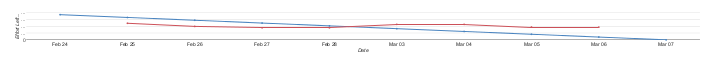
\includegraphics{ch/projectManagement/fig/sprint3burndown.png}
\caption{Sprint 3 burndown chart}
\label{fig:sprint3burndown}
\end{figure}

\subsubsection{Sprint backlog}

The backlog and time usage result.

\begin{table}[H]
	\begin{tabular}{|l|p{7cm}|p{2.2cm}|p{1.5cm}|p{1.5cm}|}%
		\hline \bfseries User story & \bfseries Details & \bfseries Hours\newline estimated & \bfseries Hours spent & \bfseries Hours left
		\csvreader[head to column names]{ch/projectManagement/sec/sprint3/userstories.csv}{}% use head of csv as column names
		{\\\hline \id & \title & \estimated & \spent & \left} \\\hline% specify your coloumns here
	\end{tabular}
    \caption{Sprint 3 backlog}
\end{table}


\subsubsection{Sprint end}